
\section{Principal Components Analysis in R}

There are two functions in R for carrying out PCA - \lstinline!princomp()! and
\lstinline!prcomp()!. The \lstinline!princomp()! function uses the
\lstinline!eigen()! function to carry out the analysis on the covariance
matrix or correlation matrix, while \lstinline!prcomp()! carries out an
equivalent analysis, starting from a data matrix, using a technique called
singular value decomposition (SVD). The SVD routine has greater numerical
accuracy, so the |prcomp()| function should generally be preferred. The
\lstinline!princomp()! function is also useful when you don't have access to
the original data, but you do have a covariance or correlation matrix (a
frequent situation when re-analyzing data from the literature). We'll concentrate on using the |prcomp()| function.


\subsection{Bioenv dataset}
To demonstrate PCA we'll use a dataset called `bioenv.txt' (see class wiki), obtained from a book called ``Biplots in Practice'' (M. Greenacre, 2010). Here is Greenacre's description of the dataset:

\begin{quote}
  The context is in marine biology and the data consist of two sets of variables observed at the same locations on the sea-bed: the first is a set of biological variables, the counts of five groups of species, and the second is a set of four environmental variables. The data set, called ``bioenv'', is shown in Exhibit 2.1. The species groups are abbreviated as ``a'' to ``e''. The environmental variables are ``pollution'', a composite index of pollution combining measurements of heavy metal concentrations and hydrocarbons; depth, the depth in metres of the sea-bed where the sample was taken; ``temperature'', the temperature of the water at the sampling point; and ``sediment'', a classification of the substrate of the sample into one of three sediment categories.
\end{quote}

The first column has no header, and corresponds to the site labels.
%
\begin{R}
> b <- read.delim('bioenv.txt',row.names=1) # note use of row.names argument
[1] "a"           "b"           "c"           "d"           "e"
[6] "Pollution"   "Depth"       "Temperature" "Sediment"
\end{R}

The columns labeled `a' to `e' contain the counts of the five species at each site.  We'll work with this abundance data for now.
%
\begin{R}
> abund <- subset(b, select=c(a,b,c,d,e))
> boxplot(abund, xlab="Species", ylab="Counts", main="Distribution of\nSpecies Counts per Site")
\end{R}

From the boxplot it looks like the counts for species `e' are smaller on average, and less variable. The mean and variance functions confirm that.
%
\begin{R}
> apply(abund,2,mean)
        a         b         c         d         e
13.466667  8.733333  8.400000 10.900000  2.966667
> apply(abund,2,var)
        a         b         c         d         e
157.63678  83.44368  73.62759  44.43793  15.68851
\end{R}


A correlation matrix suggests weak to moderate associations between the variables, but the scatterplot matrix generated by the |chart.Correlation()| function suggests that many of the relationships have a strong non-linear element.
%
\begin{R}
> cor(abund)
           a           b           c            d            e
a  1.0000000  0.67339954 -0.23992888  0.358192050  0.273522301
b  0.6733995  1.00000000 -0.08041947  0.501834036  0.036914702
c -0.2399289 -0.08041947  1.00000000  0.081504483 -0.343540453
d  0.3581921  0.50183404  0.08150448  1.000000000 -0.004048517
e  0.2735223  0.03691470 -0.34354045 -0.004048517  1.000000000

> library(PerformanceAnalytics)
> chart.Correlation(abund)
\end{R}

\subsection{PCA of the Bioenv dataset}
Linearity is not a requirement for PCA, as it's simply a rigid rotation of the original data. So we'll continue with our analysis after taking a moment to read the help on the |prcomp()| function.
\begin{R}
> ?prcomp
> a.pca <- prcomp(abund, center=T, retx=T)
    # center=T mean centers the data
    # retx=T returns the PC scores
    # if you want to do PCA on correlation matrix set scale.=T
    #    -- notice the period after scale!

> summary(a.pca)
Importance of components:
                           PC1    PC2    PC3     PC4     PC5
Standard deviation     14.8653 8.8149 6.2193 5.03477 3.48231
Proportion of Variance  0.5895 0.2073 0.1032 0.06763 0.03235
Cumulative Proportion   0.5895 0.7968 0.9000 0.96765 1.00000
\end{R}
We see that approximately 59\% of the variance in the data is capture by the first PC, and approximately 90\% by the first three PCs.

Let's compare the values return by PCA to what we would get if we carried out eigenanalysis of the covariance matrix that corresponds to our data.

\begin{R}
> a.pca
Standard deviations:
[1] 14.865306  8.814912  6.219250  5.034774  3.482308

Rotation:
          PC1         PC2         PC3         PC4         PC5
a  0.81064462  0.07052882 -0.53108427  0.18442140 -0.14771336
b  0.51264394 -0.27799671  0.47711910 -0.63418946  0.17342177
c -0.16235135 -0.88665551 -0.40897655 -0.01149647  0.14173943
d  0.22207108 -0.31665237  0.56250980  0.72941223 -0.04422938
e  0.06616623  0.17696554 -0.08141111  0.17781482  0.96231977
> eigen(cov(abund))
$values
[1] 220.97732  77.70266  38.67908  25.34895  12.12647

$vectors
            [,1]        [,2]        [,3]        [,4]        [,5]
[1,]  0.81064462 -0.07052882  0.53108427  0.18442140 -0.14771336
[2,]  0.51264394  0.27799671 -0.47711910 -0.63418946  0.17342177
[3,] -0.16235135  0.88665551  0.40897655 -0.01149647  0.14173943
[4,]  0.22207108  0.31665237 -0.56250980  0.72941223 -0.04422938
[5,]  0.06616623 -0.17696554  0.08141111  0.17781482  0.96231977
\end{R}
Notice that the `rotation' object returned by the |prcomp| function are the scaled eigenvectors (scaled to have length 1). The standard deviations of the PCA are the square roots of the eigenvalues of the covariance matrix.

\subsection{Calculating Factor Loadings}

Let's calculate the `factor loadings' associated with the PCs:
\begin{R}
> V <- a.pca$rotation # eigenvectors
> L <- diag(a.pca$sdev) # diag mtx w/sqrt of eigenvalues on diag.

> a.loadings <- V %*% L
> a.loadings
        [,1]       [,2]       [,3]        [,4]       [,5]
a 12.0504801  0.6217053 -3.3029460  0.92852016 -0.5143835
b  7.6206090 -2.4505164  2.9673232 -3.19300085  0.6039081
c -2.4134024 -7.8157898 -2.5435276 -0.05788214  0.4935804
d  3.3011545 -2.7912626  3.4983893  3.67242602 -0.1540203
e  0.9835813  1.5599356 -0.5063161  0.89525751  3.3510942
\end{R}
The magnitude of the loadings is what you want to focus on. For example, species `a' and `b' contribute most to the first PC, while species `c' has the largest influence on PC2.

You can think of the loadings, as defined above, as the components (i.e lengths of the projected vectors) of the original variables with respect to the PC basis vectors.  Since vector length is proportional to the standard deviation of the variables they represent, you can think of the loadings as giving the standard deviation of the original variables with respect the PC axes. This implies that the loadings squared sum to the total variance in the original data, as illustrated below.
\begin{R}
> apply(a.loadings**2, 1, sum)
        a         b         c         d         e
157.63678  83.44368  73.62759  44.43793  15.68851
> apply(abund, 2, var)
        a         b         c         d         e
157.63678  83.44368  73.62759  44.43793  15.68851
\end{R}

\subsection{Drawing Figures to Represent PCA}

\subsubsection{PC Score Plots}

The simplest PCA figure is to depict the PC scores, i.e. the projection of the observations into the space defined by the PC axes. Let's make a figure with three subplots, depicting PC1 vs PC2, PC1 vs PC3, and PC2 vs. PC3.
\begin{R}
> par(mfrow=c(1,3))
> plot(a.pca$x[,1], a.pca$x[,2],asp=1,pch=16, xlab='PC1', ylab='PC2',xlim=c(-30,30),ylim=c(-30,30))
> plot(a.pca$x[,1], a.pca$x[,3],asp=1,pch=16, xlab='PC1', ylab='PC3',xlim=c(-30,30),ylim=c(-30,30))
> plot(a.pca$x[,2], a.pca$x[,3],asp=1,pch=16, xlab='PC2', ylab='PC3',xlim=c(-30,30),ylim=c(-30,30))
\end{R}
Note that you should always set |asp=1| when plotting PC scores, so that the distances between points are accurate representations. Note too that I used the |xlim| and |ylim| arguments to keep the axis limits the same in all plots; comparable scaling of axes is important when comparing plots. Also note the use of the |mfrow| argument to |par()| in order to setup a multicolumn plot.

\begin{figure}[htbp]
\centering
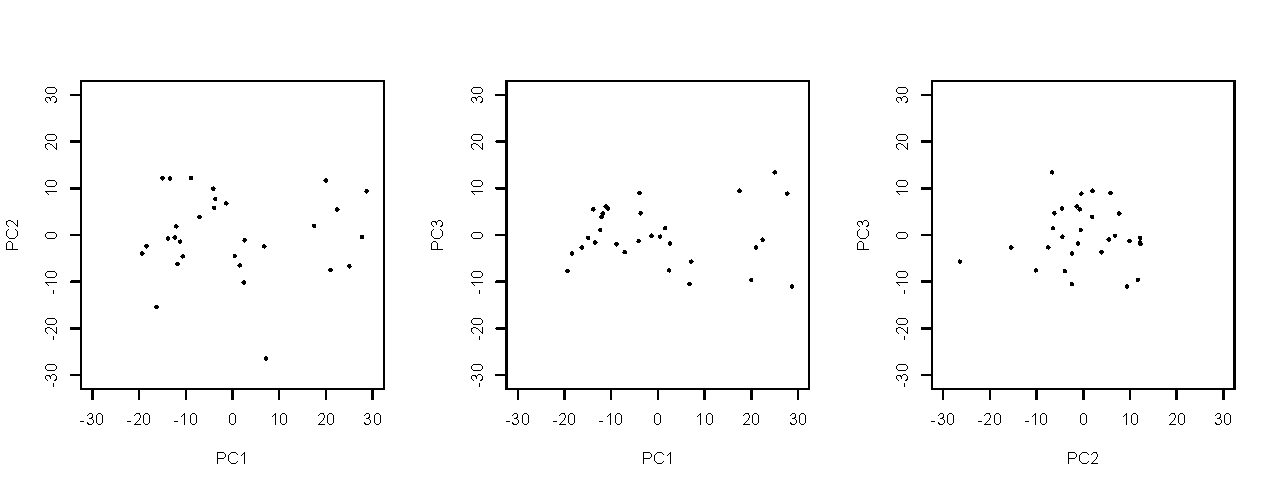
\includegraphics[width=0.95\columnwidth]{./figures/hands-on5/bioenv-scores.pdf}
\caption{Projection of the bioenv dataset into the basis defined by the first three PCs.}\label{fig:bioenvscore}
\end{figure}


As we did in previous weeks we can also use one of the 3D plotting functions to make a 3D scatterplot of the scores.
\begin{R}
> library(rgl)
> plot3d(a.pca$x[,1:3], asp=1, type='s', xlim=c(-30,30), ylim=c(-30,30), zlim=c(-30,30),col='red',size=2)
\end{R}

\subsubsection{Simultaneous Depiction of Observations and Variables in the PC Space}

Let's return to our simple PC score plot.  As we discussed above, the loadings are components of the original variables in the space of the PCs. This implies we can depict those loadings in the same PC basis that we use to depict the scores.
%
\begin{R}
> plot(a.pca$x[,1], a.pca$x[,2],asp=1,pch=16, xlab='PC1', ylab='PC2',xlim=c(-30,30),ylim=c(-30,30))

# get the loadings for each variable w/respect to PCs 1 and 2
> load2d.a <- a.loadings[1,1:2]
> load2d.b <- a.loadings[2,1:2]
> load2d.c <- a.loadings[3,1:2]
> load2d.d <- a.loadings[4,1:2]
> load2d.e <- a.loadings[5,1:2]

# draw arrows depicting loadings
> arrows(0, 0, load2d.a[1], load2d.a[2], length=0.1, col='red')
> text(load2d.a[1], load2d.a[2], 'a',col='red')
> arrows(0, 0, load2d.b[1], load2d.b[2], length=0.1, col='red')
> text(load2d.b[1], load2d.b[2], 'b',col='red')
> arrows(0, 0, load2d.c[1], load2d.c[2], length=0.1, col='red')
> text(load2d.c[1], load2d.c[2], 'c',col='red')
> arrows(0, 0, load2d.d[1], load2d.d[2], length=0.1, col='red')
> text(load2d.d[1], load2d.d[2], 'd',col='red')
> arrows(0, 0, load2d.e[1], load2d.e[2], length=0.1, col='red')
> text(load2d.e[1], load2d.e[2], 'e',col='red')
\end{R}
%
\begin{figure}[htbp]
\centering
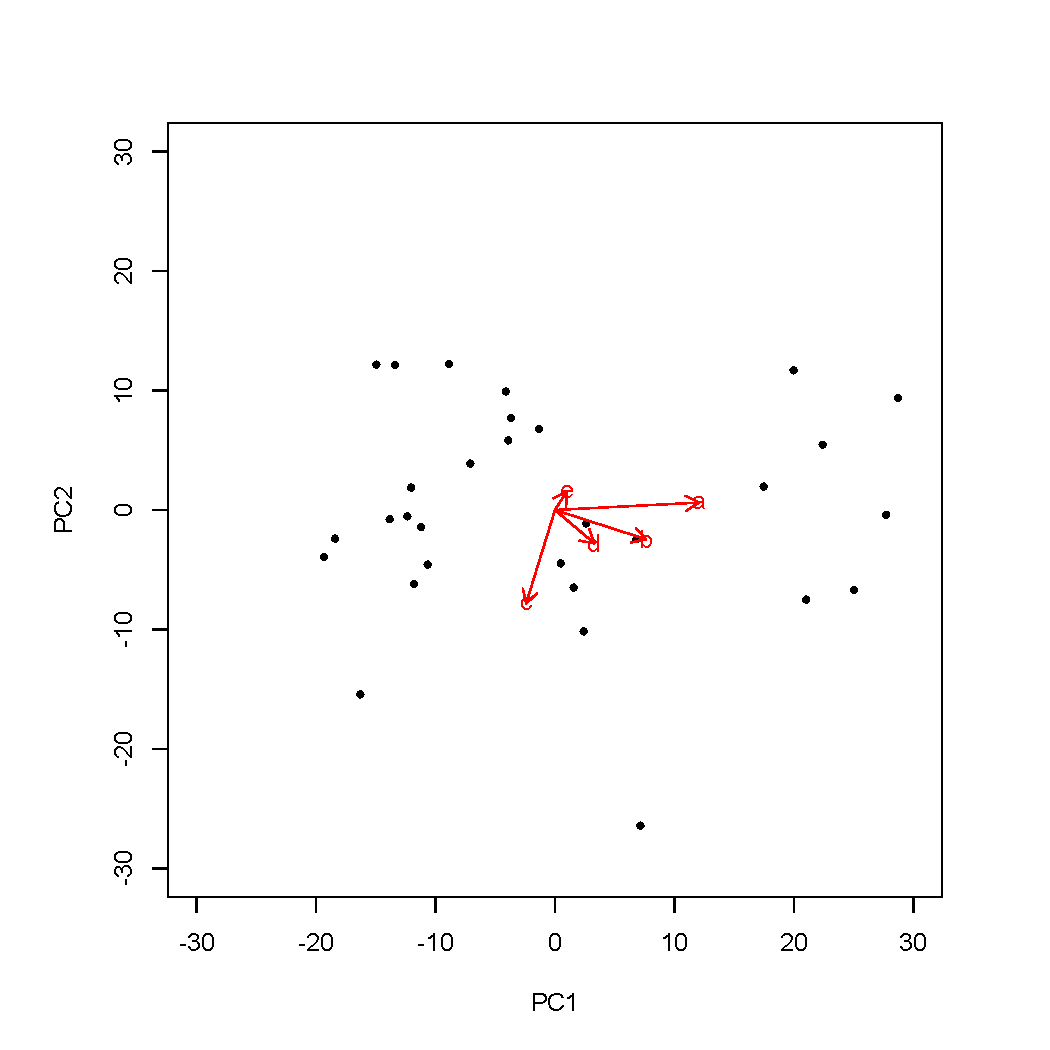
\includegraphics[width=0.5\columnwidth]{./figures/hands-on5/bioenv-simplebiplot.pdf}
\caption{PCA of the bioenv dataset. This biplot represents both the observations (black points) and variables (red vectors) in the space of PCs 1 and 2.}\label{fig:bioenvbiplot}
\end{figure}

The output of the code above should look  like Fig.~\ref{fig:bioenvbiplot}. Fig.~\ref{fig:bioenvbiplot} is called a `biplot', as it simultaneously depicts both the observations and variables in the same space.  From this biplot we can immediately see that variable `a' is highly correlated with PC1, but only weakly associated with PC2. Conversely, variable `c' is strongly correlated with PC2 but only weakly so with PC1. We can also approximate the correlations among the variables themselves -- for example `b' and `d' are fairly strongly correlated, but weakly correlated with `c'.  Keep in mind however that with respect to the relationships among the variables, this visualization is a 2D projection of a 5D space so the geometry is approximate.

The biplot is a generally useful tool for multivariate analyses and there are a number of different ways to define biplots. We'll study biplots more formally in a few weeks after we've covered singular value decomposition.



\bigskip

\begin{assignment}
Do a PCA analysis on the iris data set with all
three species pooled together. Generate a plot showing the projection of
the specimens on the first two PC axes as shown in \cref{fig:pca}.
Represent the specimens from a given species with different colors. Make
sure you include a legend for your plot.
\end{assignment}

\begin{figure}[htbp]
\centering
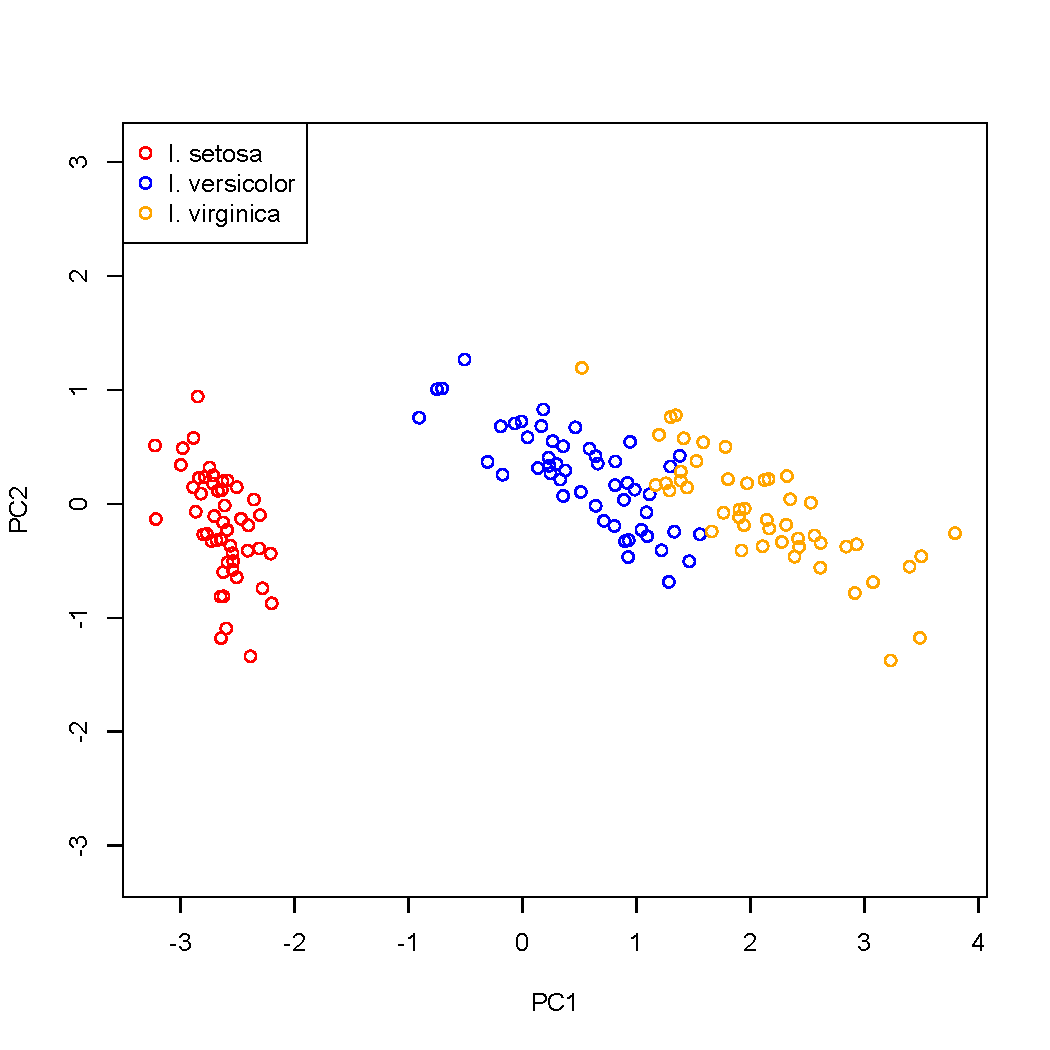
\includegraphics[width=0.5\columnwidth]{./figures/hands-on5/iris-all-pca.pdf}
\caption{PCA of the iris data set. One of your assignments is to
reconstruct this figure on your own.}\label{fig:pca}
\end{figure}

